\documentclass[9pt]{IEEEtran}

\usepackage[english]{babel}
\usepackage{graphicx}
\usepackage{epstopdf}
\usepackage{fancyhdr}
\usepackage{amsmath}
\usepackage{amsthm}
\usepackage{amssymb}
\usepackage{url}
\usepackage{array}
\usepackage{textcomp}
\usepackage{listings}
\usepackage{hyperref}
\usepackage{xcolor}
\usepackage{colortbl}
\usepackage{float}
\usepackage{gensymb}
\usepackage{longtable}
\usepackage{supertabular}
\usepackage{multicol}

\usepackage[utf8x]{inputenc}

\usepackage[T1]{fontenc}
\usepackage{lmodern}{}
\input{glyphtounicode}
\pdfgentounicode=1

\graphicspath{{./figures/}}
\DeclareGraphicsExtensions{.pdf,.png,.jpg,.eps}

% correct bad hyphenation here
\hyphenation{op-tical net-works semi-conduc-tor trig-gs}

% ============================================================================================

\title{\vspace{0ex}
Long-term tracking}

\author{Marko Medved\vspace{-4.0ex}}

% ============================================================================================

\begin{document}

\maketitle

\section{Introduction}
In this assignment, the short-term 
SiamFC tracker was adapted into a 
long-term tracking framework by using 
the peak value of the correlation 
response as an indicator of target presence. Various thresholds were tested to determine the optimal value for detecting target disappearance. The impact of the number of sampled regions on the tracker’s re-detection performance was also evaluated. Cases where the tracker successfully re-detected the target were identified and visualized. For the re-detection mechanism, uniform sampling across the entire image was initially employed, followed by an evaluation of Gaussian sampling centered around the last confident target position.


\section{Experiments}
\subsection{Short-term vs long-term tracker performance}
In the first part of the evaluation, we began by testing the short-term
 implementation of the SiamFC tracker and then compared it to the modified
  long-term version. Both trackers were evaluated on all sequences in 
  the provided dataset. The long-term modification builds on the 
  short-term tracker by introducing a thresholding mechanism based 
  on the correlation response. When the peak response falls below a
   predefined threshold, a re-detection step is triggered. This step
   samples 50 candidate positions uniformly across the entire image 
   and selects the one with the highest correlation response. The 
   re-detection process remains active until a response exceeding 
   the threshold value of 4 is found. \\
   The comparison of the trackers is presented in
    Table~\ref{tab:short_vs_long}. While the precision of 
    the long-term variant decreased slightly—possibly due to
     re-detection being unnecessarily triggered in some frames 
     where the target was still present, leading to suboptimal 
     localization—the recall and, consequently, the F-score improved
      significantly. This improvement is expected, as the short-term
       tracker typically fails to recover once the target leaves the
        field of view, whereas the long-term extension is able to
         re-detect and continue tracking.  

\begin{table}[h!]
  \centering
  \begin{tabular}{l|c|c|c}

  \textbf{Tracker} & \textbf{Precision} & \textbf{Recall} & \textbf{F-score} \\
  \hline
  Short-term & 0.5982 & 0.3251 & 0.4212 \\
  Long-term  & 0.5817 & 0.4524 & 0.5090 \\

  \end{tabular}
  \vspace{2pt}
  \caption{Performance of short-term and long-term tracking.}
  \label{tab:short_vs_long}
  \end{table}

  \subsection{Searching for the optimal value of confidence threshold}
  As previously mentioned, the maximum value of the correlation 
  response was used as a confidence score. In the initial experiments, 
  the threshold was set to 4 based on observations: the
   correlation peak typically dropped from values around 6–9 to 
   approximately 2–3 when the target was lost. The chosen 
   threshold thus fell midway between these ranges. In this 
   section, we systematically evaluate a range of thresholds 
   around this preliminary value to identify the most effective setting.
  
  On Figure~\ref{fig:thresholds} we can observe the results at different 
  thresholds. We can see that the best overall F-score is achieved with the 
  thresholds set to 4 or 5. For further evaluations we opt for 4 since it has the highest 
  F-score and this way 
  we have less unnecesary re-detections. We can see that the precision actually keeps 
  growing with a higher threshold, however the recall plummets.


  \begin{figure}[h]
    \centering
    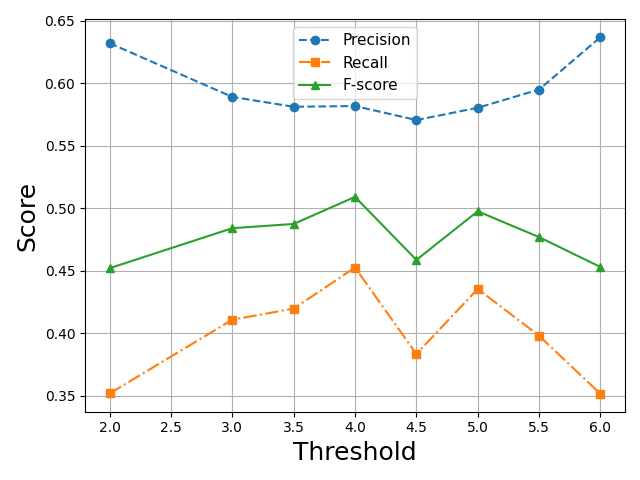
\includegraphics[width=0.99\columnwidth]{figures/thresholds.png}
    \caption{Comparison of performance at different thresholds}
    \label{fig:thresholds}
\end{figure}

\subsection{Testing different number of randomly sampled regions}
Next, we examined how the number of sampled regions during re-detection impacts 
the tracker's performance. For each sequence, we recorded the total number of frames
 required for successful re-detection, then averaged these values across all sequences.
  The results are presented in Figure~\ref{fig:samp}. Interestingly, the number of frames required 
  for re-detection does not consistently decrease as the number of sampled regions increases, which 
  would be expected if the tracker functioned perfectly. This may be due to the fact that sampling 
  more regions increases the likelihood of false positives, which can mislead the tracker and 
  ultimately delay successful re-detection.

\begin{figure}[h]
  \centering
  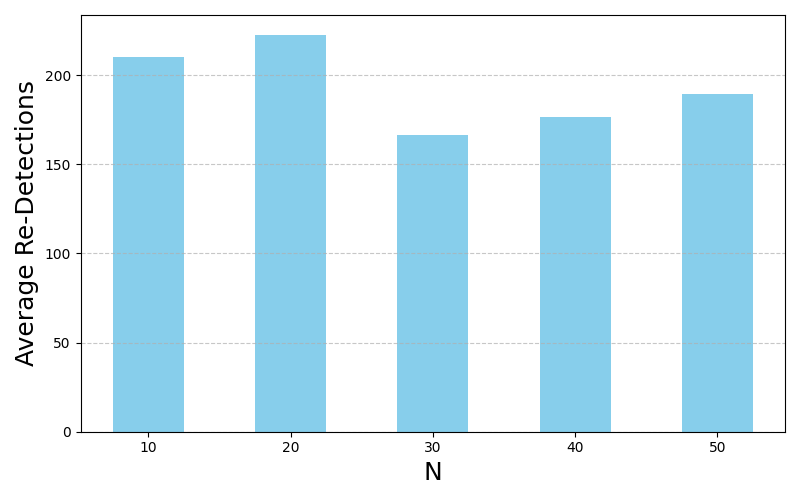
\includegraphics[width=0.99\columnwidth]{figures/diff_N.png}
  \caption{Average number of re-detection frames for different numbers of sample points}
  \label{fig:samp}
\end{figure}



\subsection{Visualization}
Here we present a visualization of the target re-detection process using our tracker, shown in Figure~\ref{fig:vis}. 
In the first image, the target is occluded by a traffic billboard, leading the tracker to lose the target and instead assign the position to a visually similar patch. 
In the second image, as the car reappears from behind the obstruction, our re-detection mechanism successfully re-identifies and tracks it.


  \begin{figure}[h]
    \centering
    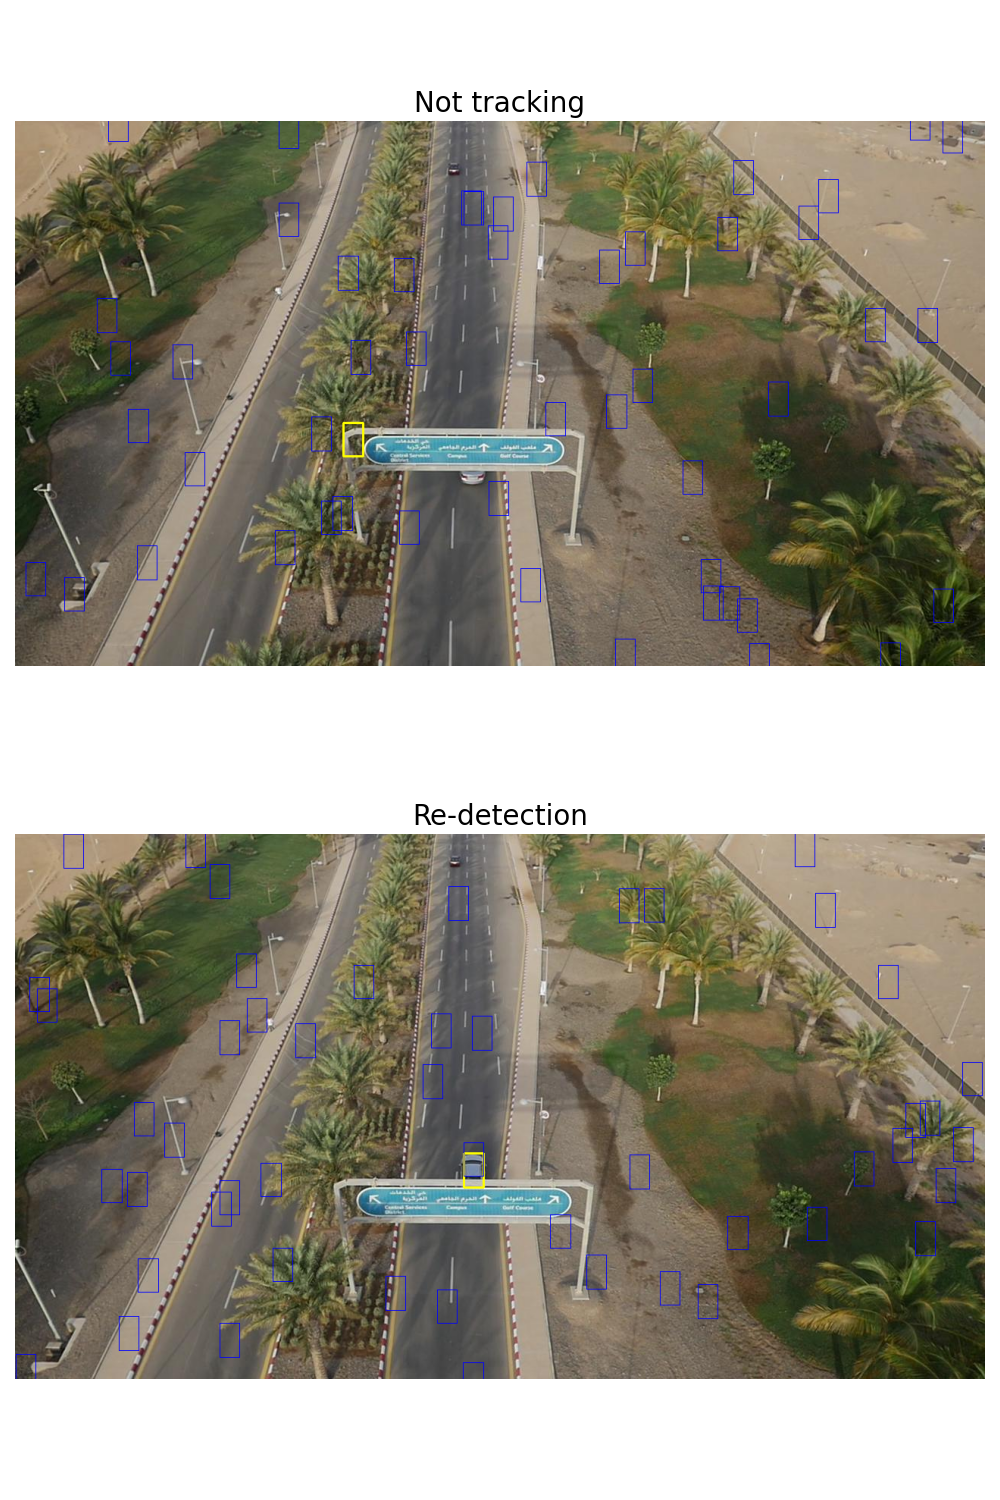
\includegraphics[width=0.99\columnwidth]{figures/vis.png}
    \caption{Example of the long term tracker re-detection}
    \label{fig:vis}
\end{figure}


\subsection{Different sampling methods}
We also tried using the gaussian sampling method, around the last confidently 
tracked point (before the correlation output was below the threshold). For this method we used 
a standard deviation of $1/10$ of the height of the image.  The results 
(Table~\ref{tab:sampling_strategies}) show a slight improvement 
in precision but a small drop in recall, with the overall F-score remaining nearly the same. This
 trade-off can be attributed to the localized nature of Gaussian sampling: the tracker becomes more 
 focused on regions near the last known location, which helps avoid false positives from distant, 
 similar-looking regions—hence the improved precision. However when the target re-appears on a completly
  different part of 
the image, the tracker with gaussian sampling is more likely to miss it, leading to reduced recall.

\begin{table}[h!]
  \centering
  \begin{tabular}{l|c|c|c}
  \textbf{Sampling Strategy} & \textbf{Precision} & \textbf{Recall} & \textbf{F-score} \\
  \hline
  Uniform  & 0.5817 & 0.4525 & 0.5090 \\
  Gaussian & 0.5971 & 0.4430 & 0.5087 \\
  \end{tabular}
  \vspace{2pt}
  \caption{Performance comparison between uniform and Gaussian sampling strategies.}
  \label{tab:sampling_strategies}
\end{table}

  

\section{Conclusion}
In this assignment we successfully modified a short-term tracker to long-term tracker and significantly
improved the performance on long-term sequences. We showed that for our implementation of 
re-detection with correlation response peaks, the optimal threshold was 4. We found out that the number 
of sampled points does not necesarily mean a faster re-detection. We showed examples 
of successfull re-detection. Lastly we tried 2 different sampling strategies: uniform accross the entire 
frame and gaussian around the last successfully tracked point with a constant standard deviation. 
We found out that both methods perform similarly. 



\bibliographystyle{IEEEtran}
\bibliography{bibliography}

\end{document}
